\chapter{MyAddedValue}
\todo{ParseTree needs to refer productions not grammar rules!!!}
\section{Text Editor}
as reasoned in \todo{REF XTEXT Conclusion} it is just possible to view the unaugmented textual serialized representations of language without potential loss of referential integrity. As a result the modeled data must be described entirely by the word. To seamlessly integrate textual languages in EMF, referential integrity must be kept. To maintain referential integrity, extrensic IDs could be added  to the token stream. The text editor must be able to handle IDs or the user editing the serialized representation must comply to a contract. A simple example is that an ID is kept unique. Allowing exactly this case might be beneficial because the double occurance of an ID indicates the semantics of a change: that one element was copied. A special integration layer between the token stream leaving the text editor and the token stream entering the model parser could handle this case. This is not always true, for example if the original element was refered and the clone can not be distingushed from the original. \\
The textual model editor must be able to handle IDs in general, not just the ones attached to lexemes. 


\section{ID Token}
\subsection{General Requirements}
The job of an ID token is to uniquely identify something in a serializeable context. 
The ideal characteristics are:
\begin{itemize}
	\item bindable and existence depedant on another token or standalone
	\item unlimited number of identifiers
	\item atomic, ID integritiy should be perserved, unbreakable
	\item standardised, long term guarantee
	\item ubiqious available
	\item abstract characters: fast distinguisable from non ID tokens
	\item private / missinterpretable / non amigious in its use
\end{itemize}

\subsection{Unicode Private-Use Characters}
A possible solution offers Unicode \cite{Unicode}. Unicode is a universal character encoding standard for consistent encoding and exchange of text data. It is the default encoding of HTML and XML and is implemented in all modern operating systems. It specifies a numeric value (code point) and name for each character. Unicode was developed in conjunction with the Universal Character Set and can be represented by widely available encodings like UTF-8. The Unicode Standard defines private-use characters, which interpretation is not specified and is determined by a private agreement among cooperative users. For example Apple uses a private character to present it's apple logo. A application specific changed interpretation of for example the character representing the apple logo is valid, as it specifies its intended behaviour according to a private agreement.\\
The private use characters are intended for softwaredevelopers. They can be compared to the ideal characteristics:
\begin{itemize}
	\item they are stand alone characters and are not bindable per se.
	\item The number of identifiers is limited to 137,468, in which 6,400 are in the private use area U+E000 to U+F8FF and 65,534 are in each supplementary private use Area-A and Area-B. 
	\item They are single characters and thus atomic. 
	\item Unicode is standardised and private-use characters are permanently designated for private use.
	\item Unicode, especially the UTF-8 enconding is wide spread and nearly ubiqious avaiable on modern personal computer platforms.
	\item There are three code-blocks for private-use characters. Three range check for a code point is in sufficient to determine its private-use.
	\item Private-use characters are, as the name states, explicitly designed for private use.
\end{itemize}

The restriction of a limited number of available identifiers could be solved by implementing a non-standard character encoding, probably a variable-with enconding.


\section{NotationModel}

\begin{figure}
\centering
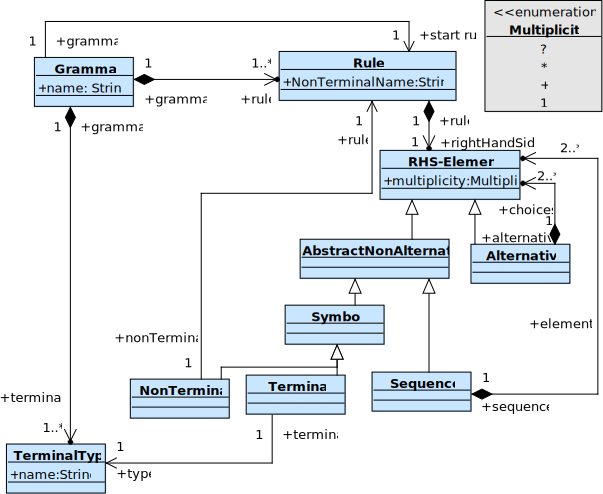
\includegraphics[scale=0.8]{gfx/ex/GrammarUML} 
\caption{EBNF Sample Grammar}
\label{MM:GrammarUML}
\end{figure}
\todo{Recreate from topcased. Lexemes now}
Figure \ref{MM:GrammarUML} shows a metamodel for an EBNF grammar. It is a reduced 

\begin{figure}
\centering
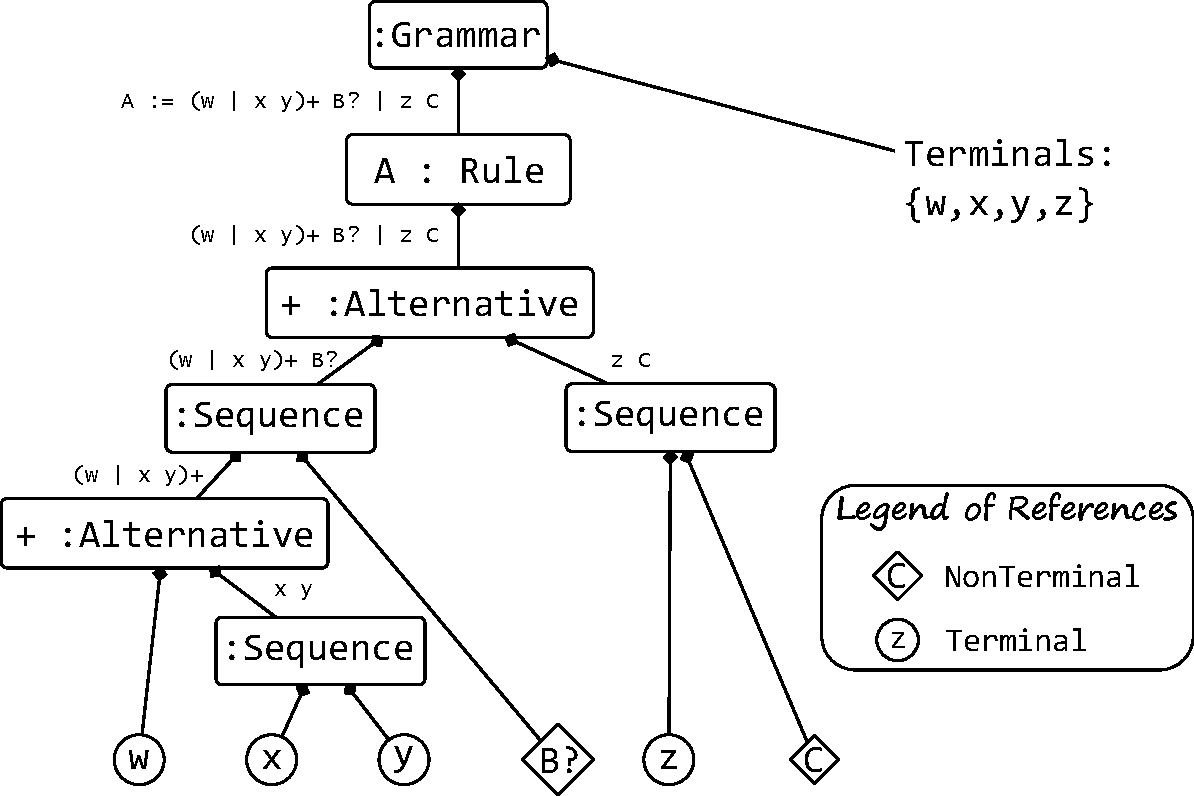
\includegraphics[scale=0.7]{gfx/ex/grammarExample} 
\caption{Example Rule ``A := (w |x y)+ B? | z C''}
\label{MM:GrammarExample}
\end{figure}
\FloatBarrier

Figure \ref{MM:GrammarExample} shows the model instance of the grammar  \code{A := (w |x y)+ B? | z C}. The grammar rules B and C are left out, as well as the start rule reference and the references to the symbols w, x, y and z are replaced with the name of the referenced symbol.


%	-------------- Latex testing --------------
The Notation model is an EMF model to describe a tree. A node or leaf contains a reference to the describing language model element.T he notation model bridges the token stream and the abstract syntax. It is the parse tree, and thus also describes a valid concrete syntax representation of the model.  It is a mandatory to updated or created it when generating a concrete representation of the model. If the notation model (element) was created to complement a language model (element), the notation model (element) serves as a disambiguis bulding plan to create the token stream for a valid concrete representation. In gereral, the notation model saves information which is not stored in the language model but relevant for presentation. It also keeps a generic, type save reference on the represented language object.\\
Each notation element represents (part of) a language element and should be a stable container for different visual representations of that element with addionaly layout information.  Due to this, if an element has multiple semantically equivalent representations, it is possible to switch the representation without switching the notation element. A switch would invalidade the descendants of the current node. A notion element therefore contains a transient structural feature containing all possible valid concrete representation rules, the non-transient last representation rule and optional the last user selected representation rule. In case these representation rules are grammar rules, they must be complemented with addionional information in order to make the token production unambigious. For example a grammar rule like:
\begin{xtxt}
A : (B | C) "myKeyword"
\end{xtxt}
would be translated to the following productions rules 
\begin{xtxt}
A - > B "myKeyword"
A - > C "myKeyword"
\end{xtxt}
for the sake of abstraction and simplicity, this distinction, especially im more complex scenarios, should be hidden from the language developer. In a case where B and C are semantically equivalent  it is arbitrary from the abstract syntax perspective if an A contains a B or C. The notation element must close this gap, so an notation element refering to a lanuage element represented by A doesn't need to store the keyword "myKeyword", this information is implicit, but it must distinguish if the concrete presentation of this particular A should use B or C as a presentation selection. It is therefore not nessecary to explicity assign  a production rule but to implicity make one resolvable by dissolving the ambiguity for options and choices which have no representation in the language model. \\
The base class for representation rules must be general, or unspecific, enough allow non textual representations. Notation elements should prefer containment references instead of attributes to easy to ease merging, like the GMF notation model. In contrast to GMF, this driving motivation is not team support but easier automatic updating between old and new versions.\\
In order to integrate with incremental parsing, notation model elements should hold a transient integer which contains the distance to the first previous token accesing the current one in it's lookahead. \\
Finally, a notation model element should contain a flag if it is currently textually visible.
\todo{ rewrites possible}
\todo{ reason that a representation in text editor is necessary}
\todo{mention that addtionaly layout information can be added to a node}

\section{Unparser}
The unparser is responsible to find all valid parse trees for the current language model. To save space and allow the user to selectivly choose for a specific element between different representations, the desired result is a compressed format of the parse forest as a directed asyclic graph (DAG).  As described in XText bla \todo{ref}, this is a CSP to find a valid assignment of grammar rules to the current language model. The currently observered implementation of XText uses backtracking with O(exp(n)) runtime to solve this problem for a particular chase. To find all possible solutions, the average runtime will likely drastically increase. Furthermore, this algorithm doesn't compress the parse forest in general. Additionally, it is strongly desireable to guide the resolution process to, e.g. Prefer user selected representations or to avoid special representations, e.g. Representations containing ID tokens. Improving the unparsers runtime is crucial for real world applications of the size of average computer programs.

\section{Use and implementation of the ID-Token}
The possible use of an ID token is twofold:
\begin{itemize}
	\item adding an ID to a token
	\item using the ID to refer an EObject
\end{itemize}
To extend the use of an ID token, it could be extended with an associatitivy: right, none or left.
It is therefore mandatory to save this addional information in an associated resource. The above restriction to an EObject ensures XMI serializablitiy. The resource should contain a map from ID token to a triple containing the associativity, the ID or UUID and an EObject). The associativity determines if it's a plain ID or as a reference token. Non associative tokens are EObject references. The second place can't be shared in case the extrensic UUID of the EObject should be preserved.

ID tokens could be implemented by wrapping the existent lexical analyser. The wrapping lexer loads the additional resource and resolves the token if it is recongized on the input strema. If a non associative ID token is resolved and regular the next token of the normal lexer is after the ID token, it is cached and the resolved ID token is returned. In case the current position on the character stream is not smaller than the positition of the ID token, the token of the regular parser is returned. In case of plain ID tokens with right associativtiy the ID is assigned to a property of the token return by the wrapped lexer. Left associative tokens require a lookahead of one regular token and should be avoided for this reason. Also, in the case the wrapping parser doesn't know about the ignored characters, this requires that it inspects the returned normal token to recongnize errors where an ID token was contained in a regular token. The primary use of an ID token is likely to let the lexer return an EObject to the parser as an atomic token.


\section{Use cases}
The definition of ID tokens, unparser and notation model don't in the previous sections just indicated their amended use. This sections describes their intergrated use and how the concepts leaverage each other. \todo{review the need of ID token handling by the editor, play scenarios to gain pages?}

\subsection{Incomplete information handling}
The first, obvious benefit of ID tokens is that the textual representation doesn't nessessarly need to describe the whole model. It enables the use of EObject directly in the grammar and thus the grammar to properly handle parts of the lanuage. The results in inablity to modify the unhandeled parts and the existence of an ID token, or a character placeholder at the unhandeled location. This shifts the problem of handling this ID token to the text editor.

\subsection{Different representations of semantic equivalent tokens}
In case the unparser found more than one valid grammar rule for a notation element, the corresponding transient field is set. The text editor should offer the user the change the current representation value, which reassigns the grammar rule of the current notation element and, if necessary, also to its decendants. As soon as the reassignment is finished, a new token stream is produced reflecting the new textual representation.


\subsection{Sententential Tokens \& Graphical Editors}
Because the notation model is the parse and consists of EObjects, it is possible to serialize notation nodes as single ID tokens. Sentential tokens are tokens which represent a sentenential production. The additional definition of sentential tokens circumvents the contradicting statement of nonterminal tokens on the input token stream. This concept is necessary for incremental parsers and can be leaveraged for visual editing. This can be used to fold parts of the word into an ID token. This ID token is completely grammar conform. The main benefit is not folding of word parts but to allow a graphical editor to be presented at the ID tokens location editing the refered language object. It is important to mention, that the editor edits a language object, but is a substitute or semantic equivalent of a specific terminal or nonterminal, or a set, but never a sequence of them. This means that the editor may edit the language object and its descendants just as long as the unparser allows one of the editors semantic equivalents at the current position. If the graphical editor nests textual representation, it must create an own parser instance. This parser instance can be of the same type as the outer parser instance with a different start symbol, but doesn't has to be. It must be sychronized to the same language model. It might also reuse the noation model, which is guaranteed if a new instance of the outer parser is used.

\todo{annotation special} \\
\todo{ reason about factory methods} \\
\todo {sententential tokens as generated grammar productions} \\
\todo{each notation model element as stateless edit part} \\